\documentclass[11pt]{amsart}

\usepackage{amsmath,amsthm}
\usepackage{amssymb}
\usepackage{graphicx}
\usepackage{enumerate}
\usepackage{fullpage}
 \usepackage{euscript}
% \makeatletter
% \nopagenumbers
\usepackage{verbatim}
\usepackage{color}
\usepackage{hyperref}

\usepackage{csvsimple}

\usepackage{fullpage,tikz,float}
\usepackage{tikz-cd}
%\usepackage{times} %, mathtime}

\textheight=600pt %574pt
\textwidth=480pt %432pt
\oddsidemargin=15pt %18.88pt
\evensidemargin=18.88pt
\topmargin=10pt %14.21pt

\parskip=1pt %2pt

% define theorem environments
\newtheorem{theorem}{Theorem}    %[section]
%\def\thetheorem{\unskip}
\newtheorem{proposition}[theorem]{Proposition}
%\def\theproposition{\unskip}
\newtheorem{conjecture}[theorem]{Conjecture}
\def\theconjecture{\unskip}
\newtheorem{corollary}[theorem]{Corollary}
\newtheorem{lemma}[theorem]{Lemma}
\newtheorem{sublemma}[theorem]{Sublemma}
\newtheorem{fact}[theorem]{Fact}
\newtheorem{observation}[theorem]{Observation}
%\def\thelemma{\unskip}
\theoremstyle{definition}
\newtheorem{definition}{Definition}
%\def\thedefinition{\unskip}
\newtheorem{notation}[definition]{Notation}
\newtheorem{remark}[definition]{Remark}
% \def\theremark{\unskip}
\newtheorem{question}[definition]{Question}
\newtheorem{questions}[definition]{Questions}
%\def\thequestion{\unskip}
\newtheorem{example}[definition]{Example}
%\def\theexample{\unskip}
\newtheorem{problem}[definition]{Problem}
\newtheorem{exercise}[definition]{Exercise}

\numberwithin{theorem}{section}
\numberwithin{definition}{section}
\numberwithin{equation}{section}

\def\reals{{\mathbb R}}
\def\torus{{\mathbb T}}
\def\integers{{\mathbb Z}}
\def\rationals{{\mathbb Q}}
\def\naturals{{\mathbb N}}
\def\complex{{\mathbb C}\/}
\def\distance{\operatorname{distance}\,}
\def\support{\operatorname{support}\,}
\def\dist{\operatorname{dist}\,}
\def\Span{\operatorname{span}\,}
\def\degree{\operatorname{degree}\,}
\def\kernel{\operatorname{kernel}\,}
\def\dim{\operatorname{dim}\,}
\def\codim{\operatorname{codim}}
\def\trace{\operatorname{trace\,}}
\def\dimension{\operatorname{dimension}\,}
\def\codimension{\operatorname{codimension}\,}
\def\nullspace{\scriptk}
\def\kernel{\operatorname{Ker}}
\def\p{\partial}
\def\Re{\operatorname{Re\,} }
\def\Im{\operatorname{Im\,} }
\def\ov{\overline}
\def\eps{\varepsilon}
\def\lt{L^2}
\def\curl{\operatorname{curl}}
\def\divergence{\operatorname{div}}
\newcommand{\norm}[1]{ \|  #1 \|}
\def\expect{\mathbb E}
\def\bull{$\bullet$\ }
\def\det{\operatorname{det}}
\def\Det{\operatorname{Det}}
\def\rank{\mathbf r}
\def\diameter{\operatorname{diameter}}

\def\t2{\tfrac12}

\newcommand{\abr}[1]{ \langle  #1 \rangle}

\def\newbull{\medskip\noindent $\bullet$\ }
\def\field{{\mathbb F}}
\def\cc{C_c}



% \renewcommand\forall{\ \forall\,}

% \newcommand{\Norm}[1]{ \left\|  #1 \right\| }
\newcommand{\Norm}[1]{ \Big\|  #1 \Big\| }
\newcommand{\set}[1]{ \left\{ #1 \right\} }
%\newcommand{\ifof}{\Leftrightarrow}
\def\one{{\mathbf 1}}
\newcommand{\modulo}[2]{[#1]_{#2}}

\def\bd{\operatorname{bd}\,}
\def\cl{\text{cl}}
\def\nobull{\noindent$\bullet$\ }

\def\scriptf{{\mathcal F}}
\def\scriptq{{\mathcal Q}}
\def\scriptg{{\mathcal G}}
\def\scriptm{{\mathcal M}}
\def\scriptb{{\mathcal B}}
\def\scriptc{{\mathcal C}}
\def\scriptt{{\mathcal T}}
\def\scripti{{\mathcal I}}
\def\scripte{{\mathcal E}}
\def\scriptv{{\mathcal V}}
\def\scriptw{{\mathcal W}}
\def\scriptu{{\mathcal U}}
\def\scriptS{{\mathcal S}}
\def\scripta{{\mathcal A}}
\def\scriptr{{\mathcal R}}
\def\scripto{{\mathcal O}}
\def\scripth{{\mathcal H}}
\def\scriptd{{\mathcal D}}
\def\scriptl{{\mathcal L}}
\def\scriptn{{\mathcal N}}
\def\scriptp{{\mathcal P}}
\def\scriptk{{\mathcal K}}
\def\scriptP{{\mathcal P}}
\def\scriptj{{\mathcal J}}
\def\scriptz{{\mathcal Z}}
\def\scripts{{\mathcal S}}
\def\scriptx{{\mathcal X}}
\def\scripty{{\mathcal Y}}
\def\frakv{{\mathfrak V}}
\def\frakG{{\mathfrak G}}
\def\aff{\operatorname{Aff}}
\def\frakB{{\mathfrak B}}
\def\frakC{{\mathfrak C}}

\def\symdif{\,\Delta\,}
\def\mustar{\mu^*}
\def\muplus{\mu^+}

\def\soln{\noindent {\bf Solution.}\ }


%\pagestyle{empty}
%\setlength{\parindent}{0pt}

\begin{document}

\begin{center}{\bf CS294 Deep Reinforcement Learning --- UCB, Spring 2017 --- William}
\\
{\bf Homework 1, Behavioral Cloning}
\end{center}
\textbf{Task 2.1}. Behavioral cloning on one successfull and one one unsuccessfull task.
\begin{figure}[H]
	 \begin{tabular}{l|ccccc}%
	 \hline
    \bfseries Algorithm &  Task & $ E(t_{end})$ & $ \bar{r}$ & \bfseries$\sigma(r)$% specify table head
    \csvreader[head to column names]{fig1.csv}{}% use head of csv as column names
    {\\\hline\alg  &  \task & \error & \avgr & \stdr}% specify your coloumns here
    \\\hline
    \end{tabular}
    \medskip
    \caption{The results from behavioral cloning on two different tasks against an expert.}
\end{figure}
\emph{Details for Figure 2.} The blcone algorithm was a neural network  $\scriptn$ with a 400 neuron ReLu layer followed by a 300 neuron ReLu layer followed by a $m$ neuron linear layer where $m$ denotes the size of the action space of the task. The network  $\scriptn$  was trained by minimizing $E: (s,y) \mapsto \|\scriptn(s) - y\|^2$ for expert actions $y$ drawn from a trajectory distribution generated by some expert policy $\pi: \scripts \to \scripta$ with $\scripts$ the state space and $\scripta$ the action space for the Humanoid-v1 task. Batches of size 64 were fed to bclone every time step $t \in \{ 1, \cdots, N\}$.  The $E(t_{end})$ column yields the testing error of $E$ accross the entire expert policy training set after the training the neural network on $N = 10000$ batches from a replay buffer of size $N$. In this comparison there were $10$ rollouts to accumulate data. The $\hat{r}$ and $\sigma(r)$ columns denote the testing return (mean and standard devation respectively) over $20$ testing rollouts of $\scriptn$. In this experiment behavioral cloning on Ant-v1 but not Humanoid-v0. 

\newpage 

\medskip \noindent \textbf{Task 2.3}. Behavorial cloning against a hyperparameter. 

\begin{figure}[H]
	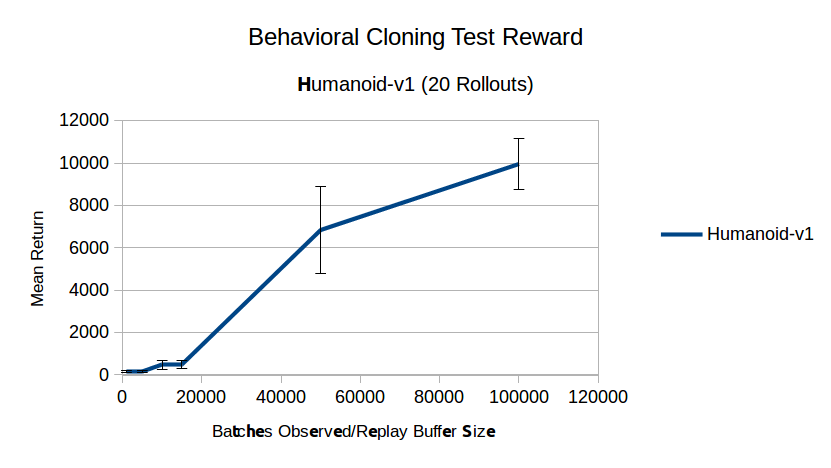
\includegraphics[width=0.8\textwidth]{dagger_fig_2.png}
	 \begin{tabular}{l|cccccc}%
	 \hline
    \bfseries Algorithm & \bfseries $R$ & \bfseries $N$ & \bfseries $\epsilon$ & $ E(t_{end})$ & $ \bar{r}$ & \bfseries$\sigma(r)$% specify table head
    \csvreader[head to column names]{fig2.csv}{}% use head of csv as column names
    {\\\hline\alg  & \roll &\iters & \lr & \ee & \avgr & \stdr}% specify your coloumns here
    \\\hline
    \end{tabular}
    \medskip
    \caption{{The results from varying the the number of observed rollouts, $N$, that the behavioral cloning algorithm observes.}}
\end{figure}


    \emph{Details for Figure 2.} The blcone algorithm was a neural network  $\scriptn$ with the same network architecture as that described in Task 2.2. The network  $\scriptn$  was trained by minimizing $E: (s,y) \mapsto \|\scriptn(s) - y\|^2$ for expert actions $y$ drawn from a trajectory distribution generated by some expert policy $\pi: \scripts \to \scripta$ with $\scripts$ the state space and $\scripta$ the action space for the Humanoid-v1 task. Batches of size 64 were fed to bclone every time step $t \in \{ 1, \cdots, N\}$.  The $E(t_{end})$ column yields the testing error of $E$ accross the entire expert policy training set after the coressponding number of batches in the $N$ coilumn. The $\epsilon$ column denotes the learning rate of $\scriptn$. The $\hat{r}$ and $\sigma(r)$ columns denote the testing return (mean and standard devation respectively) over $20$ testing rollouts of $\scriptn$.

    This particular hyperparaemter was chosen for experimentation as it stands to reason that more time learning directly on the expert policy (with more data) will lead a more general cloned policy. Although varying this hyperaparameter in general lead to more successful rollouts, the variance of these rollouts was significantly higher as cloned policy $\scriptn$ often diverged from the state-action trajectory distribution of the expert.

\newpage
\medskip \noindent \textbf{Task 3.2}. DAgger as an improvement to behavioral cloning.

    \begin{figure}[H]
    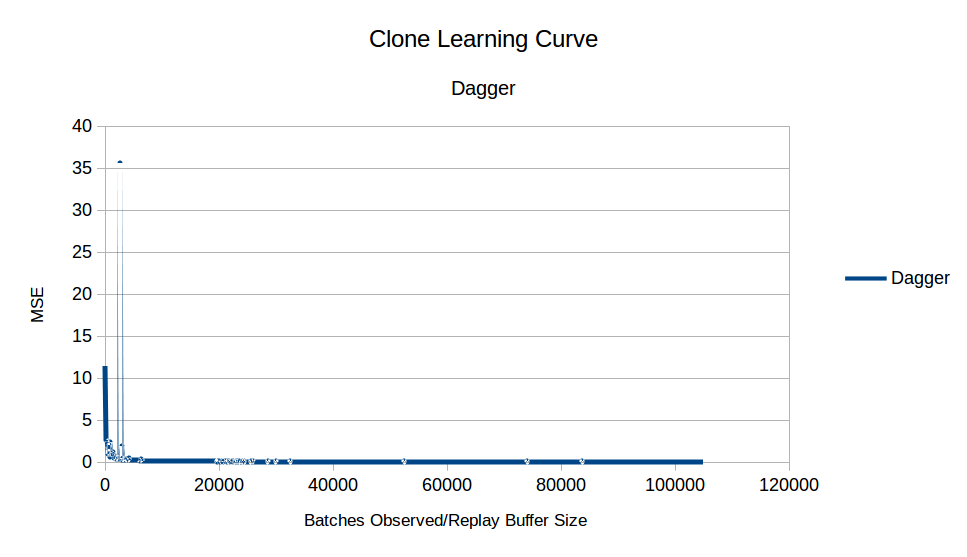
\includegraphics[width=0.49\textwidth]{dagger_clone_learning.png}
    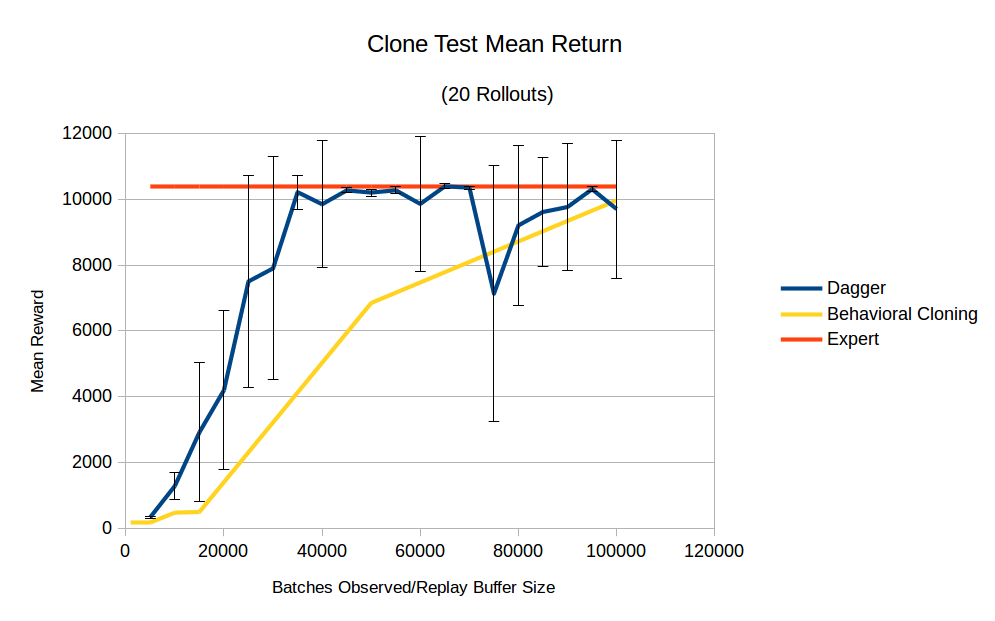
\includegraphics[width=0.49\textwidth]{dagger_clone_test.png}
    \caption{(Left) A plot of the clone mean squared error curve using dagger on Humanoid-v1. (Right) A comparison of the clone test mean reward as the number of learning iterations (and datapoints) increase on the same task.}
    \end{figure}
    \emph{Details for Figure 3.} The blcone algorithm was a neural network  $\scriptn$ with the same network architecture as that described in Task 2.2. The network  $\scriptn$  was trained by minimizing $E: (s,y) \mapsto \|\scriptn(s) - y\|^2$ for expert actions $y$ generated by some expert policy $\pi: \scripts \to \scripta$ with $s \in \scripts$ the state space and $a \in \scripta$ the action space for the Humanoid-v1 task. \textbf{However}, at every iteration the action taken was $\scriptn(s)$ and \textbf{not} $\pi(s)$, the action of the expert policy\footnote{This is the essential setp of the DAgger algorithm.}.  Batches size, learning rate, and evaluation metrics are the exact same as Figure 2.

    In the above Figure, it is clear that providing expert labels for states generated by $\scriptn$ avoids the disribution mismatch problem, and at $N \simeq 45,000$ we have that $\scriptn$ achieves the not only the same average return as $\pi$ but also the same standard deviation $\sigma(r).$ Beyond this point we suspect $\scriptn$ began to overfit to the replay buffer, but further investigation is required.
 
\end{document}\end
	